\documentclass[border=55pt]{standalone}

\usepackage{tikz}
\usepackage{xcolor}
\usepackage{graphicx}
\usepackage{amsmath}

\usetikzlibrary{arrows.meta}

\begin{document}
\begin{tikzpicture}[scale=1, transform shape]
    \newlength{\borderdim}
    \setlength{\borderdim}{0.9mm}%
    \newlength{\photodim}
    \setlength{\photodim}{5.0cm}%
    \node[
        circle,
        draw=gray!30,
        inner sep=0,
        minimum size=\photodim,
        line width=\borderdim,
        path picture={
            \node at (path picture bounding box.center){
                    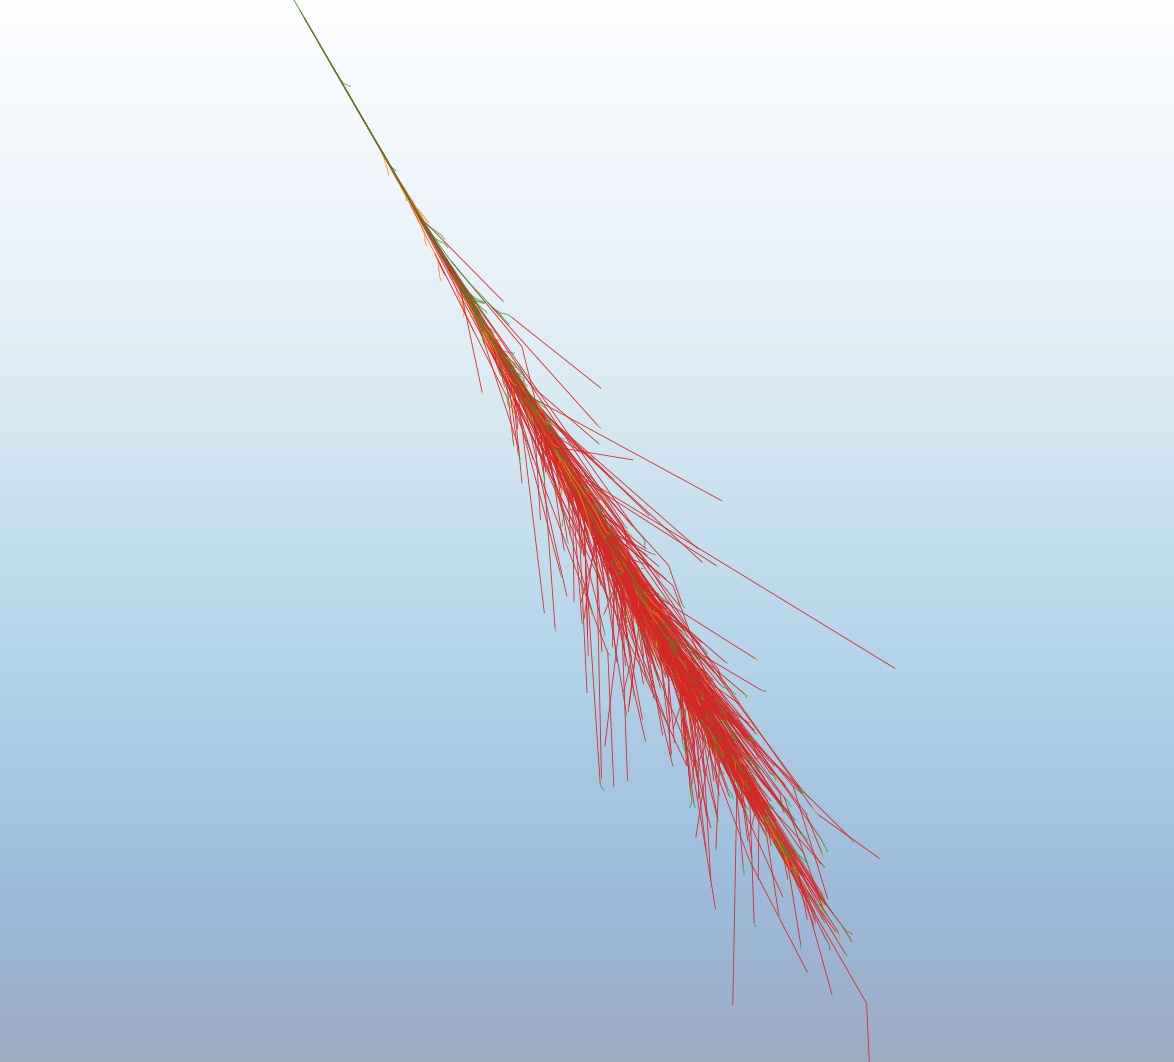
\includegraphics[width=5.5cm]{./corsika_shower/build/shower.jpg}
                };
        }] (A) {};

    \node[
        circle,
        draw=gray!30,
        inner sep=0,
        minimum size=\photodim,
        line width=\borderdim,
        path picture={
            \node at (path picture bounding box.center){
                    \includegraphics[width=4.5cm]{./neuronal_network/network.jpg}
                };
        }] (B) at (4,4) {};

    \node[
        circle,
        draw=gray!30,
        inner sep=0,
        minimum size=\photodim,
        line width=\borderdim,
        ] (C) at (8,0) {
            \texttt{est.} = $\begin{pmatrix}
                \texttt{Energy}\\
                \texttt{direction}\\
                \texttt{type}
            \end{pmatrix}$
        };

    \draw [
        -Stealth,
        rounded corners=0.4cm,
        draw=gray,
        thick,
        shorten <= 0.5cm,
        shorten >= 0.5cm
        ] (A.north) -- (0,4) -- (B.west);

    \draw [
        -Stealth,
        rounded corners=0.4cm,
        draw=gray,
        thick,
        shorten <= 0.5cm,
        shorten >= 0.5cm
        ] (B.east) -- (8,4) -- (C.north);

\end{tikzpicture}

\end{document}
